\subsection{Hamiltonian Cycles}

\begin{definition}\label{1.11}
    A \textbf{Hamiltonian cycle}\index{Hamiltonian cycle} in a graph $G$ is a spanning subgraph that is a cycle (isomorphic to $C_n$ for some $n\in\mathbb{N}$)\\
    If $G$ has a Hamiltonian cycle, $G$ is called \textbf{Hamiltonian} 
\end{definition}

\vspace{0.5cm}

\begin{theorem}[Dirac's Theorem]\label{1.12}
    Let $G$ be a graph of order $n\geq 3$ where the \textbf{order}\index{order} of $G$ is given by $|V(G)|$ and the \textbf{size} by $|E(G)|$. If every Vertex of $G$ has degree at least $\frac{n}{2}$ then $G$ is Hamiltonian 
\end{theorem}

\vspace{0.5cm}

\begin{theorem}[Ore's theorem]\label{1.13}
    Let $G$ be a graph of order $n\geq3$. If for every pair $u,v\in V,u\neq v,u$ and $v$ non-adjacent, we have $\deg(u)+\deg(v)\geq n$ then $G$ is Hamiltonian
\end{theorem}
\begin{remark}\label{1.14}
\hfill \\
    Ore $\implies$ Dirac
\end{remark}
\begin{proof}
    \begin{itemize}
    \hfill \\
        \item The Graph $G$ is connected: suppose $G$ is not connected. Take an arbitrary component of $G$ and call it $H$. The order of $H$ is $n-k$ if $k$ vertices are not in $V(H)$. Now any $v\in V(H)$ has $\deg(v)\leq n-k-1$ with equality if $v$ is adjacent to every vertex in $V(H)$. Now take $u\notin V(H)$ so $\deg(u)\leq k-1$. It follows that $u,v\in V(G),u\neq v$ and $u,v$ are not adjacent so $\deg(u)+\deg(v)\geq n$ but $\deg(u)+\deg(v)\leq k-1+n-k-1=n-2<n$ $\lightning$
        \item $G$ has a Hamiltonian cycle: By induction on the number of non-edges
        \item No non-edge $\implies G$ complete, hence Hamiltonian
        \item Assume $G$ non complete $u,v\in V, u\neq v$, be non-adjacent. By induction the graph $G'$ obtained from $G$ by adding $e=\{u,v\}$ as an edge is Hamiltonian. Let~$C$ be a Hamiltonian cycle of $G'$. If $C$ does not use $e\implies C$ is Hamiltonian cycle in $G$. Assume $C$ uses $e$. Removing $e$ from $C$ yields a path from $u$ to $v$\par
        For $i\in\{2,...,n-1\}$
        \item If $v_i$ is a neighbour of $u$, color $\{v_{i-1},v_i\}$ red
        \item If $v_i$ is a neighbour of $v$, color $\{v_{i},v_{i+1}\}$ blue
        \item Since $\deg(u)+\deg(v)\geq n$ and the path $v_1,...,v_n$ has $n-1$ edges, there exists an edge $\{v_{i},v_{i+1}\}$ which is both red and blue. Then $v_1,...v_i,v_n,v_{n-1},...,v_{i+1}$ is a Hamiltonian cycle in $G$.
    \end{itemize}
    \begin{center}
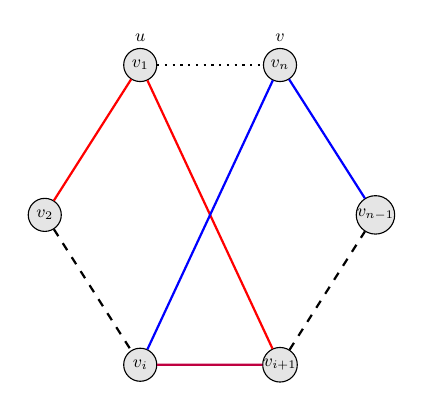
\begin{tikzpicture}[ scale=0.7,
    vertex/.style={circle, draw, fill=gray!20, minimum size=6mm, inner sep=0pt},
    every node/.style={font=\small, transform shape}
]
\def\r{3}
\node[vertex] (v1)  at ({90-335}:\r)            {$v_1$};
\node[vertex] (vn)  at ({90-25}:\r)         {$v_n$};
\node[vertex] (vi)  at ({90-205}:\r)        {$v_i$};
\node[vertex] (vi1) at ({90-155}:\r)        {$v_{i+1}$};
\node[vertex] (v2) at ({90-270}:\r)        {$v_2$};
\node[vertex] (vn1)  at ({0}:\r)        {$v_{n-1}$};

\draw[thick, red] (v1)--(v2);
\draw[thick, blue] (vn)--(vn1);
\draw[thick, dotted] (v1)--(vn);
\draw[thick, dashed] (v2)--(vi);
\draw[thick, dashed] (vi1)--(vn1);
\draw[thick, purple] (vi)--(vi1); 
\draw[thick, red] (v1)--(vi1);
\draw[thick, blue] (vn)--(vi);

% Labels for u and v
\node[above=3mm] at (v1)  {$u$};
\node[above=3mm]  at (vn)  {$v$};

\end{tikzpicture}
\end{center}
\end{proof}